% Staggered Grid Structure of the Discrete Cosserat Rod
% Companion document to system-formulation.tex

\documentclass[11pt]{article}

% ---------------------------------------------------------------------------
% Font and encoding
% ---------------------------------------------------------------------------
\usepackage{palatino}
\usepackage[T1]{fontenc}
\usepackage[utf8]{inputenc}

% ---------------------------------------------------------------------------
% Page layout
% ---------------------------------------------------------------------------
\usepackage[top=1in, bottom=1in, left=1.25in, right=1.25in]{geometry}
\usepackage{setspace}
\setstretch{1.15}
\setlength{\parindent}{1em}
\setlength{\parskip}{0.4em}

% ---------------------------------------------------------------------------
% Math
% ---------------------------------------------------------------------------
\usepackage{amsmath}
\usepackage{amssymb}
\usepackage{bm}

% ---------------------------------------------------------------------------
% Figures and tables
% ---------------------------------------------------------------------------
\usepackage{graphicx}
\usepackage{booktabs}
\usepackage{float}

% ---------------------------------------------------------------------------
% Colors and hyperlinks
% ---------------------------------------------------------------------------
\usepackage{xcolor}
\usepackage[hidelinks]{hyperref}

% ---------------------------------------------------------------------------
% Lists
% ---------------------------------------------------------------------------
\usepackage{enumitem}
\setlist[itemize]{nosep, topsep=0.3em, itemsep=0.2em}

% ---------------------------------------------------------------------------
% Section formatting
% ---------------------------------------------------------------------------
\usepackage{titlesec}
\titlespacing*{\section}{0pt}{1.2em}{0.6em}
\titlespacing*{\subsection}{0pt}{0.9em}{0.3em}

% ---------------------------------------------------------------------------
% Custom commands
% ---------------------------------------------------------------------------
\newcommand{\vect}[1]{\mathbf{#1}}
\newcommand{\mat}[1]{\mathbf{#1}}
\newcommand{\Real}{\mathbb{R}}

% ---------------------------------------------------------------------------
\begin{document}
% ---------------------------------------------------------------------------

\begin{center}
  {\Large\bfseries Staggered Grid Structure of the Discrete Cosserat Rod} \\[0.5em]
  {\large Nodes, Elements, and Voronoi Nodes} \\[1.5em]
  \textit{Snake-HRL Project --- Reference Document}
\end{center}

\vspace{1em}

% ===================================================================
\section{Overview}
% ===================================================================

The continuous Cosserat rod is discretized on a \textbf{staggered grid} with three interleaved layers of discrete points.
This document explains what each layer stores, how they relate to each other, and how the sparse matrix operators move information between them.

\begin{figure}[H]
  \centering
  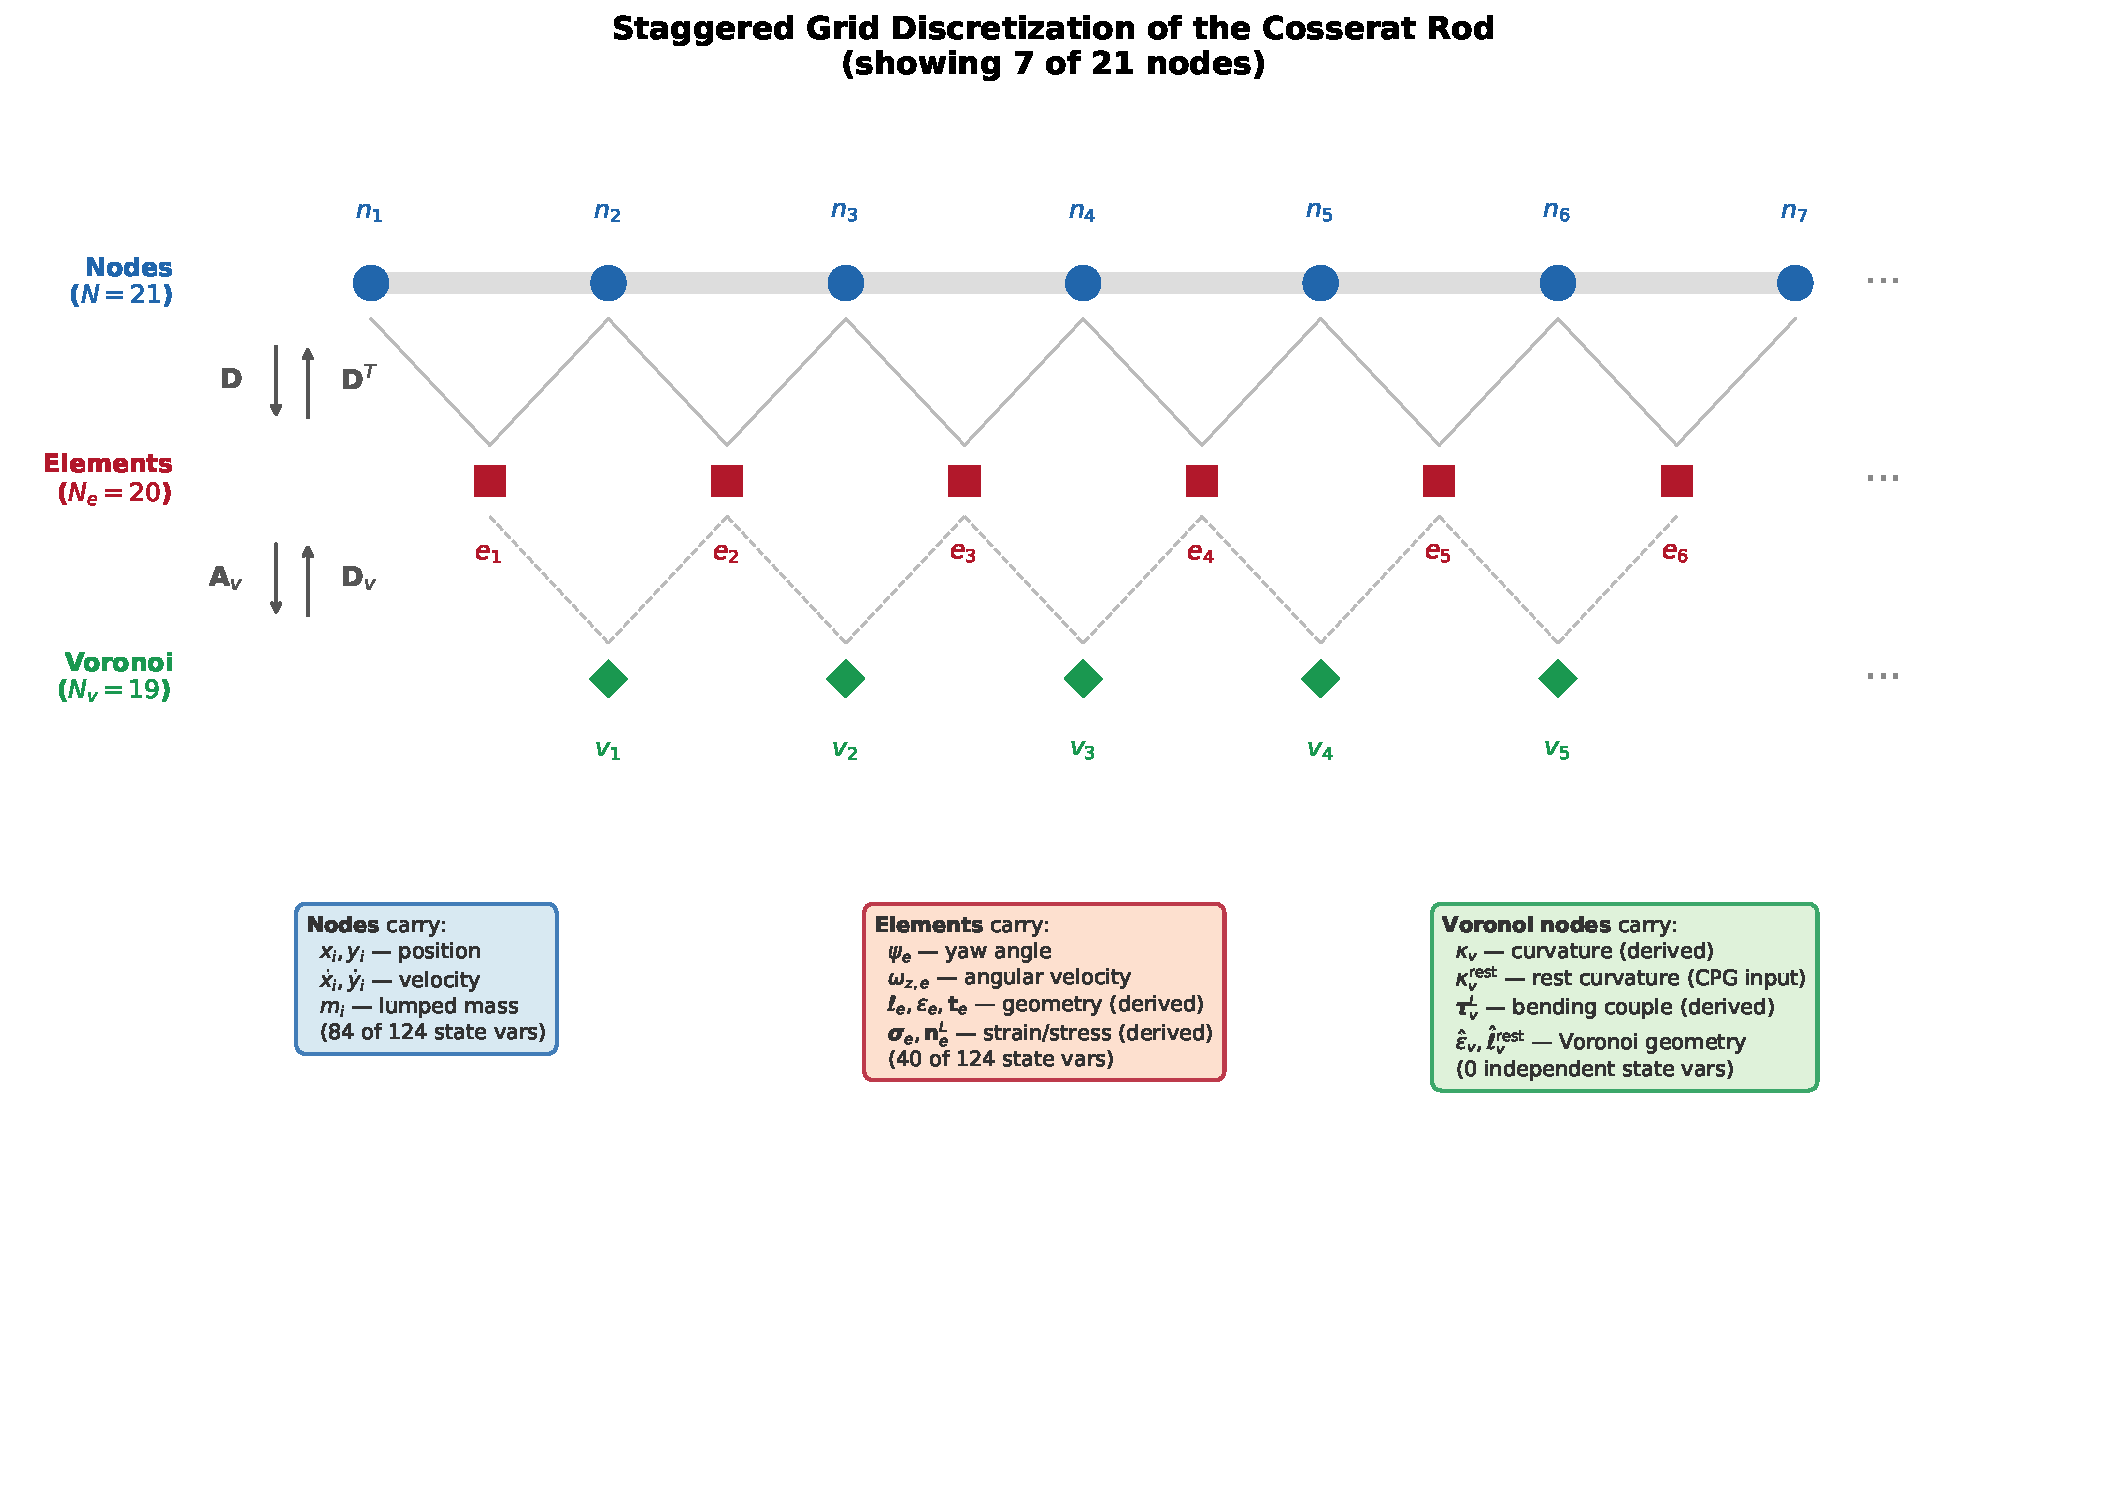
\includegraphics[width=\textwidth]{../figures/staggered_grid.pdf}
  \caption{The three-layer staggered grid.
    Nodes (blue circles) sit at the rod vertices; elements (red squares) span between adjacent nodes; Voronoi nodes (green diamonds) sit between adjacent elements.
    Arrows on the left show the matrix operators that transfer information between layers.}
  \label{fig:staggered-grid}
\end{figure}

% ===================================================================
\section{The Three Layers}
% ===================================================================

% -------------------------------------------------------------------
\subsection{Nodes ($i = 1, \ldots, N$; $N = 21$)}
% -------------------------------------------------------------------

Nodes are the \textbf{vertices} of the rod.
They are the primary spatial discretization points and carry all \textbf{translational} degrees of freedom.

\paragraph{Stored quantities.}
\begin{itemize}
  \item $x_i, y_i \in \Real$ --- position of node $i$ in the plane
  \item $\dot{x}_i, \dot{y}_i \in \Real$ --- translational velocity of node $i$
  \item $m_i \in \Real$ --- lumped mass (interior nodes: $\rho A \, \ell^{\text{rest}} \approx 1.88 \times 10^{-4}$\,kg; boundary nodes: half that)
\end{itemize}

\paragraph{Physical meaning.}
Node positions $\{(x_i, y_i)\}_{i=1}^{N}$ trace out the rod centerline.
The straight-line segment between two adjacent nodes is an \emph{element}.
Lumped masses are computed by assigning each node the mass of its adjacent half-elements: interior nodes carry two half-elements, boundary nodes carry one.

\paragraph{Indexing.}
$i = 1$ is the tail and $i = 21$ is the head of the snake (or vice versa, depending on convention).
Together, the $N = 21$ nodes carry $21 \times 2 = 42$ position scalars and $21 \times 2 = 42$ velocity scalars, totaling \textbf{84 of the 124 state variables}.

% -------------------------------------------------------------------
\subsection{Elements ($e = 1, \ldots, N_e$; $N_e = 20$)}
% -------------------------------------------------------------------

Elements are the \textbf{segments} connecting adjacent nodes.
Element $e$ spans from node $e$ to node $e+1$.
They carry all \textbf{rotational} degrees of freedom and all quantities that describe the \emph{local deformation} of the rod.

\paragraph{Stored quantities.}
\begin{itemize}
  \item $\psi_e \in \Real$ --- yaw angle (orientation of element $e$ in the plane)
  \item $\omega_{z,e} \in \Real$ --- angular velocity about the vertical axis
  \item $\ell_e \in \Real$ --- current length: $\ell_e = \|\vect{x}_{e+1} - \vect{x}_e\|$
  \item $\varepsilon_e \in \Real$ --- dilatation (axial stretch): $\varepsilon_e = \ell_e / \ell_e^{\text{rest}}$
  \item $\vect{t}_e \in \Real^2$ --- unit tangent vector: $\vect{t}_e = (\vect{x}_{e+1} - \vect{x}_e) / \ell_e$
  \item $\bm{\sigma}_e \in \Real^2$ --- generalized strain in the local (material) frame
  \item $\vect{n}_e^L \in \Real^2$ --- internal stress: $\vect{n}_e^L = \mat{S}\,(\bm{\sigma}_e - \bm{\sigma}_e^{\text{rest}})$
  \item $\mat{Q}_e \in \Real^{2 \times 2}$ --- rotation matrix: entries $\cos\psi_e$, $\sin\psi_e$
\end{itemize}

\paragraph{Physical meaning.}
Each element is a rigid segment with orientation $\psi_e$.
The difference between an element's actual configuration and its rest configuration produces the \emph{strain}, which the constitutive law converts to \emph{stress} (internal forces).
The rotation matrix $\mat{Q}_e$ transforms between the local (material) frame and the global (lab) frame.

\paragraph{Indexing.}
Element $e$ connects node $e$ and node $e+1$.
The $N_e = 20$ elements carry $20$ yaw angles and $20$ angular velocities, totaling \textbf{40 of the 124 state variables}.

\paragraph{Derived from nodes.}
The element length $\ell_e$, tangent $\vect{t}_e$, and dilatation $\varepsilon_e$ are \emph{not} independent state --- they are recomputed from node positions at every substep via:
\begin{equation}
  \Delta\vect{x}_e = \mat{D}\,\vect{x} = \vect{x}_{e+1} - \vect{x}_e, \qquad
  \ell_e = \|\Delta\vect{x}_e\|, \qquad
  \vect{t}_e = \Delta\vect{x}_e / \ell_e, \qquad
  \varepsilon_e = \ell_e / \ell_e^{\text{rest}}
\end{equation}

% -------------------------------------------------------------------
\subsection{Voronoi Nodes ($v = 1, \ldots, N_v$; $N_v = 19$)}
% -------------------------------------------------------------------

Voronoi nodes sit at the \textbf{midpoints between adjacent elements}.
Voronoi node $v$ sits between elements $e = v$ and $e = v + 1$.
They are the natural location for computing \textbf{curvature} (the rate of change of orientation along the rod).

\paragraph{Stored quantities.}
\begin{itemize}
  \item $\kappa_v \in \Real$ --- discrete curvature at Voronoi node $v$ (from director differences)
  \item $\kappa_v^{\text{rest}} \in \Real$ --- rest curvature (\textbf{the CPG control input} from Eq.~(8) in the system formulation)
  \item $\bm{\tau}_v^L \in \Real$ --- bending--twist couple: $\tau_v^L = B\,(\kappa_v - \kappa_v^{\text{rest}})$
  \item $\hat{\varepsilon}_v \in \Real$ --- Voronoi dilatation: average of adjacent element dilatations
  \item $\hat{\ell}_v^{\text{rest}} \in \Real$ --- Voronoi rest length: average of adjacent rest lengths ($= 0.05$\,m for uniform rod)
\end{itemize}

\paragraph{Physical meaning.}
Curvature measures how sharply the rod bends at a given point.
At Voronoi node $v$, the curvature $\kappa_v$ is computed from the angle difference between elements $v$ and $v+1$ divided by the Voronoi length.
The \textbf{rest curvature} $\kappa_v^{\text{rest}}$ is the key control input: the CPG sets this at each RL step to produce the serpentine wave that drives locomotion.
When $\kappa_v \neq \kappa_v^{\text{rest}}$, the constitutive law produces a bending moment that drives the rod toward the commanded shape.

\paragraph{Indexing.}
Voronoi node $v$ sits between elements $v$ and $v+1$ (equivalently, at the location of node $v+1$).
There are $N_v = N_e - 1 = 19$ Voronoi nodes.

\paragraph{Derived from elements.}
Voronoi quantities are computed from element quantities via the averaging operator $\mat{A}_v$:
\begin{equation}
  \hat{\varepsilon}_v = \mat{A}_v\,\bm{\varepsilon} = \tfrac{1}{2}(\varepsilon_v + \varepsilon_{v+1}), \qquad
  \hat{\ell}_v^{\text{rest}} = \tfrac{1}{2}(\ell_v^{\text{rest}} + \ell_{v+1}^{\text{rest}})
\end{equation}

% ===================================================================
\section{Interaction Between Layers}
% ===================================================================

The four sparse matrix operators move information between layers:

\begin{table}[H]
  \centering
  \renewcommand{\arraystretch}{1.3}
  \begin{tabular}{cllll}
    \toprule
    Operator & Direction & Size & Structure & Physical role \\
    \midrule
    $\mat{D}$ & Node $\to$ Element & $20 \times 21$ & Bidiagonal & Position differences $\to$ strain \\
    $\mat{D}^T$ & Element $\to$ Node & $21 \times 20$ & Bidiagonal & Internal stress $\to$ nodal forces \\
    $\mat{A}_v$ & Element $\to$ Voronoi & $19 \times 20$ & Tridiagonal & Element averages $\to$ curvature \\
    $\mat{D}_v$ & Voronoi $\to$ Element & $20 \times 19$ & Bidiagonal & Bending couple gradient $\to$ element torques \\
    \bottomrule
  \end{tabular}
  \caption{Sparse operators connecting the three layers.  Each has $O(N)$ nonzero entries.}
  \label{tab:operators}
\end{table}

\noindent
Explicitly, the difference operator is:
\begin{equation}
  \mat{D} =
  \begin{pmatrix}
    -1 & +1 &    &        &    \\
       & -1 & +1 &        &    \\
       &    & -1 & \ddots &    \\
       &    &    & \ddots & +1 \\
  \end{pmatrix}
  \in \Real^{20 \times 21}
  \label{eq:D-explicit}
\end{equation}

% ===================================================================
\section{Node Coupling Pattern}
% ===================================================================

\begin{figure}[H]
  \centering
  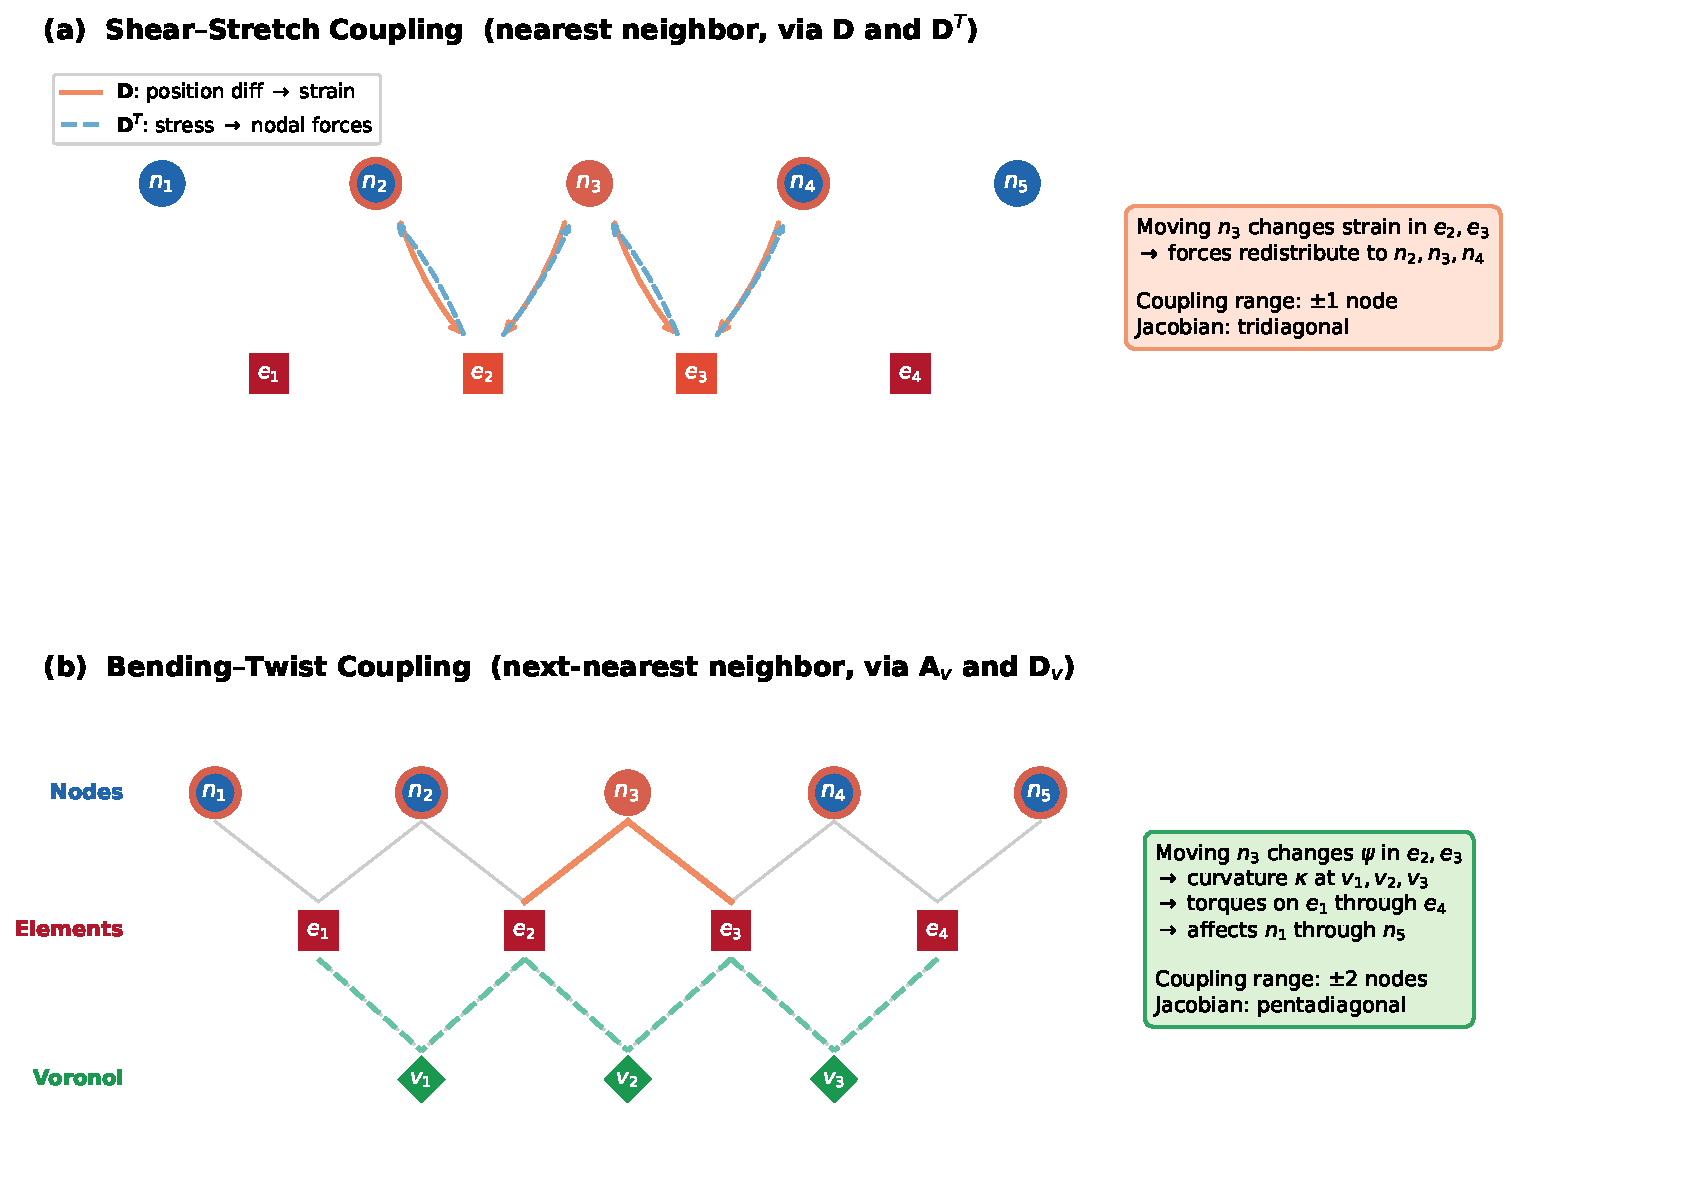
\includegraphics[width=\textwidth]{../figures/coupling_pattern.pdf}
  \caption{How adjacent nodes interact through the staggered grid.
    \textbf{(a)} Shear--stretch coupling is nearest-neighbor: moving node $n_3$ changes the strain in elements $e_2$ and $e_3$, which changes forces on nodes $n_2$, $n_3$, and $n_4$.
    \textbf{(b)} Bending--twist coupling is next-nearest-neighbor: the curvature at Voronoi nodes $v_1$, $v_2$, $v_3$ depends on elements $e_1$ through $e_4$, which depend on nodes $n_1$ through $n_5$.}
  \label{fig:coupling}
\end{figure}

\subsection{Shear--Stretch: Nearest Neighbor}

When node $i$ moves, it changes the position difference $\Delta\vect{x}$ in the two adjacent elements ($e_{i-1}$ and $e_i$).
This changes the strain and stress in those elements, which $\mat{D}^T$ distributes as forces to nodes $i-1$, $i$, and $i+1$:

\begin{equation}
  n_i \;\xrightarrow{\mat{D}}\; (e_{i-1}, e_i)
    \;\xrightarrow{\text{constitutive}}\; (\vect{n}_{i-1}^L, \vect{n}_i^L)
    \;\xrightarrow{\mat{D}^T}\; (n_{i-1}, n_i, n_{i+1})
\end{equation}

\noindent
The coupling range is \textbf{1 node} in each direction.
The resulting force Jacobian $\partial \vect{F}^{\text{int}} / \partial \vect{x}$ is \textbf{tridiagonal} (bandwidth 1).

\subsection{Bending--Twist: Next-Nearest Neighbor}

When node $i$ moves, it changes the yaw of elements $e_{i-1}$ and $e_i$.
The curvature at each Voronoi node depends on the yaw \emph{difference} of its two adjacent elements, so Voronoi nodes $v_{i-2}$, $v_{i-1}$, and $v_i$ are all affected.
The bending couple gradient ($\mat{D}_v$) then distributes torques to elements $e_{i-2}$ through $e_{i+1}$, which affect nodes $e_{i-2}$ through $e_{i+2}$:

\begin{equation}
  n_i \;\xrightarrow{\mat{D}}\; (e_{i-1}, e_i)
    \;\xrightarrow{\mat{A}_v}\; (v_{i-2}, v_{i-1}, v_i)
    \;\xrightarrow{\mat{D}_v}\; (e_{i-2}, \ldots, e_{i+1})
    \;\xrightarrow{\mat{D}^T}\; (n_{i-2}, \ldots, n_{i+2})
\end{equation}

\noindent
The coupling range is \textbf{2 nodes} in each direction.
The resulting torque Jacobian $\partial \vect{m}^{\text{int}} / \partial \vect{x}$ is \textbf{pentadiagonal} (bandwidth 2).

\subsection{Combined Jacobian Sparsity}

The overall Jacobian of the right-hand side $\partial\dot{\vect{s}}/\partial\vect{s}$ is \textbf{banded} with bandwidth at most 2 (in terms of node indices).
This means each of the 124 state variables depends on at most $\sim$10 other state variables (its own node, 2 neighbors on each side, plus the corresponding velocities and yaw angles).

This spatial locality is a key property that makes neural surrogate approximation feasible: the network does not need to learn arbitrary long-range correlations.

% ===================================================================
\section{State Variable Summary}
% ===================================================================

\begin{table}[H]
  \centering
  \renewcommand{\arraystretch}{1.3}
  \begin{tabular}{llccc}
    \toprule
    Layer & DOF & Count & Per-entity & Total \\
    \midrule
    Nodes ($N = 21$) & Positions $x_i, y_i$ & 21 & 2 & 42 \\
                      & Velocities $\dot{x}_i, \dot{y}_i$ & 21 & 2 & 42 \\
    \midrule
    Elements ($N_e = 20$) & Yaw angles $\psi_e$ & 20 & 1 & 20 \\
                           & Angular velocities $\omega_{z,e}$ & 20 & 1 & 20 \\
    \midrule
    Voronoi ($N_v = 19$) & \multicolumn{4}{l}{\textit{(no independent state --- derived from nodes and elements)}} \\
    \midrule
    \multicolumn{4}{l}{\textbf{Total state variables}} & \textbf{124} \\
    \bottomrule
  \end{tabular}
  \caption{State variables by layer.  Voronoi nodes carry derived quantities only --- they add no independent degrees of freedom.}
  \label{tab:state-summary}
\end{table}

% ---------------------------------------------------------------------------
\end{document}
